
\section{Proposed methods}

\begin{frame}[plain]
   \sectionpage
\end{frame}

\frame{
   \frametitle{From the literature}

   \textbf{\citet{mankowska2014}}
   \begin{itemize}
      \item MIP model
      \item VNS-based meta-heuristic (deterministic moves)
   \end{itemize}

   \vspace*{32pt}

   \textbf{\citet{lasfargeas2019}}
   \begin{itemize}
      \item Several variations of a constructive heuristic
      \item VNS-based meta-heuristic (randomized moves)
   \end{itemize}

   \begin{tikzpicture}[overlay]
      \node at (12,4) {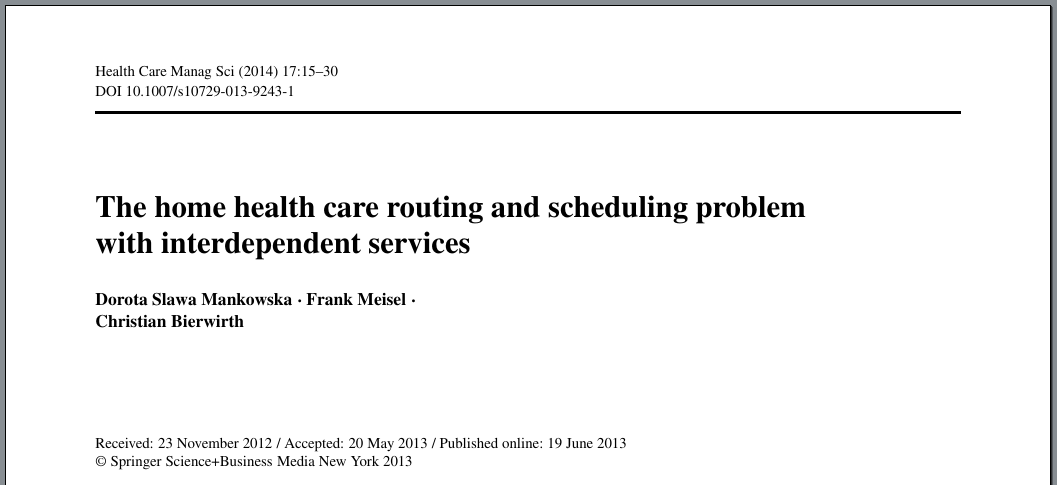
\includegraphics[scale=0.13]{fig/mankowska2014-paper.png}};
      \node at (12,1) {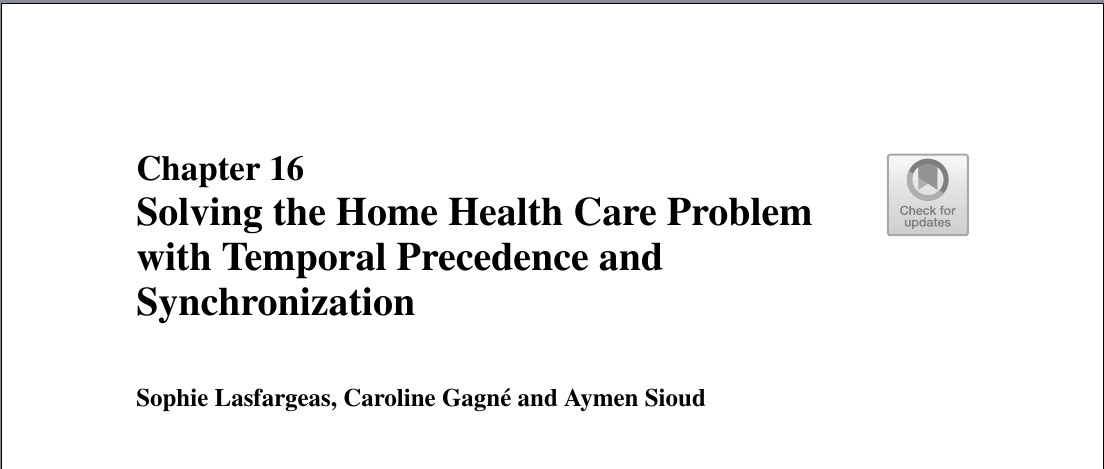
\includegraphics[scale=0.12]{fig/lasfargeas2019-paper.png}};
   \end{tikzpicture}
}

%\frame{
%   \frametitle{MIP-based methods}
%
%   \textbf{Lower bounds with CPLEX}
%   \begin{itemize}
%      \item In \citet{mankowska2014}: CPLEX 12.3 --- June, 2011
%      \item Our experiment: CPLEX 20.1 --- December, 2020
%      \begin{itemize}
%         \item Pre-processing
%         \item Parameter setting
%         \item MIP warmstart
%      \end{itemize}
%   \end{itemize}
%}

\frame{
   \frametitle{MIP-based methods}

   \textbf{Fix and optimize matheuristic}
   \begin{itemize}
      \item Initial solution: constructive heuristic \citep{mankowska2014}
      \item Each iteration: optimizes pair of routes
      \item Stop criteria: \# iterations without improvement
   \end{itemize}

   \vspace{12pt}

   \centering
   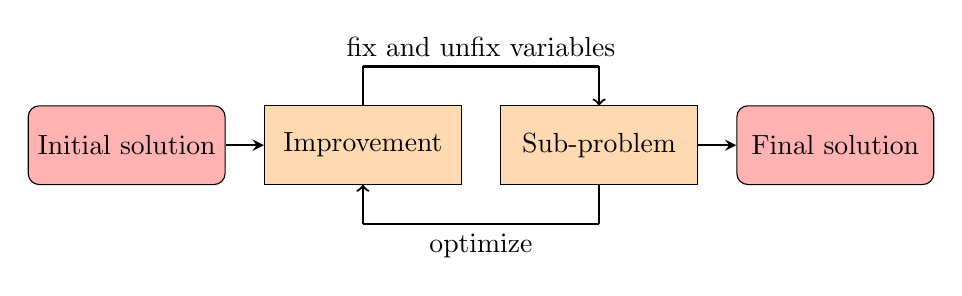
\begin{tikzpicture}[node distance=3cm]
%      \begin{adjustbox}{width=0.02\textwidth}
      \tikzstyle{startstop} = [rectangle, rounded corners, minimum width=2.5cm, minimum height=1cm,text centered, draw=black, fill=red!30]
      \tikzstyle{process} = [rectangle, minimum width=2.5cm, minimum height=1cm, text centered, draw=black, fill=orange!30]
      \tikzstyle{arrow} = [thick,->,>=stealth]

      \node (start) [startstop] {Initial solution};
      \node (pro1) [process, right of=start] {Improvement};
      \node (pro2) [process, right of=pro1] {Sub-problem};
      \node (end) [startstop, right of=pro2] {Final solution};

      \draw [arrow] (start) -- (pro1);
      \draw [arrow] (pro2) -- (end);


      \draw[thick,-] (3,1) -- (6,1) node [pos=0.5, above] {fix and unfix variables};
      \draw[thick,->] (6,1) -- (6,.5);
      \draw[thick,-] (3,1) -- (3,.5);

      \draw[thick,-] (3,-1) -- (6,-1) node [pos=0.5, below] {optimize};
      \draw[thick,-] (6,-1) -- (6,-.5);
      \draw[thick,->] (3,-1) -- (3,-.5);
%      \end{adjustbox}
   \end{tikzpicture}
}

\frame{
   \frametitle{Indirect search methods}

   \textbf{Local search-based methods can be expensive}
   \begin{itemize}
      \item Tricks from VRPTW literature reduce effort of evaluating moves
      \item But the synchronization constraints are too impacting
      \item Requires updating large chunks of the solution
   \end{itemize}

   \vspace*{18pt}

   \textbf{Our proposal:} indirect search \citep{drexl2012}
}


\frame{
   \frametitle{Indirect search methods}

   \textbf{BRKGA}
   \begin{itemize}
      \item Main concept by \citet{bean1994}
      \item Most popular version by \citet{gonccalves2011art}
   \end{itemize}

   \vspace*{18pt}

   \textbf{Intensification components}
   \begin{itemize}
      \item Island model (also in \citet{toso2015})
      \item Multi-parent mating
      \item Implicit path relinking on random keys space
      \item Proposed by \citet{andrade2021}
   \end{itemize}

   \begin{tikzpicture}[overlay]
      \node at (11.6,1.8) {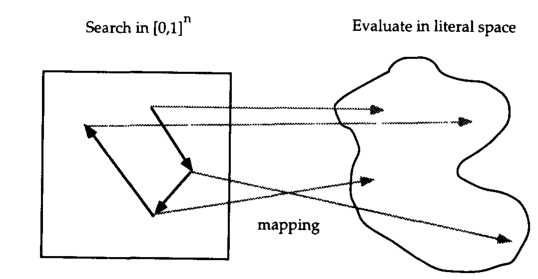
\includegraphics[scale=0.6]{fig/bean1994-rkga-decode.pdf}};
   \end{tikzpicture}
}

%\frame{
%   \frametitle{Indirect search methods}
%
%   \textbf{For the home health care problem}
%   \begin{itemize}
%      \item BRKGA $\Rightarrow$ gives a \textit{permutation} of the patients/nodes
%%      \item The proposed decoder \textit{embeds} a greedy heuristic
%      \item A \emph{best-insertion heuristic decoder} builds a routing solution from the permutation
%   \end{itemize}
%
%%   \vspace*{12pt}
%
%%   \textbf{In short:} TAS $\approx$ permutation of nodes
%
%
%
%%   \begin{figure}
%%      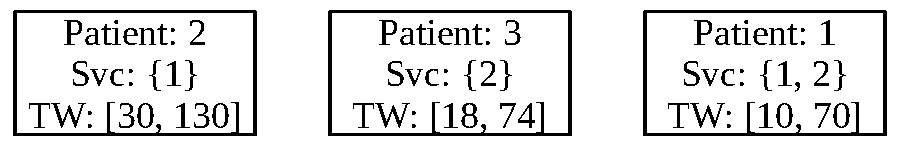
\includegraphics[width=0.5\textwidth]{fig/decoder-tis}
%%   \end{figure}
%}

